% Two rational Cauchy sequences trapped in a shrinking tube. They name the same real.
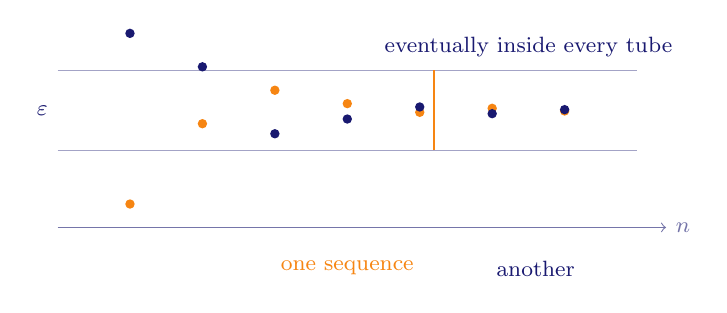
\begin{tikzpicture}[x=0.92cm,y=0.85cm]
  \draw[->,MidnightBlue!60] (0,0)--(8.4,0) node[right,font=\footnotesize] {$n$};
  \draw[MidnightBlue!40] (0,1.15)--(8,1.15);
  \draw[MidnightBlue!40] (0,2.35)--(8,2.35);
  \node[left,font=\footnotesize,MidnightBlue] at (0,1.75) {$\varepsilon$};
  \foreach \n/\y in {1/0.35,2/1.55,3/2.05,4/1.85,5/1.72,6/1.78,7/1.74}{
    \fill[BurntOrange] (\n,\y) circle (1.7pt);
  }
  \foreach \n/\y in {1/2.9,2/2.4,3/1.4,4/1.62,5/1.8,6/1.7,7/1.76}{
    \fill[MidnightBlue] (\n,\y) circle (1.7pt);
  }
  \draw[BurntOrange,thick] (5.2,1.15)--(5.2,2.35);
  \node[below,font=\footnotesize,BurntOrange] at (4,-0.35) {one sequence};
  \node[below,font=\footnotesize,MidnightBlue] at (6.6,-0.35) {another};
  \node[font=\footnotesize,MidnightBlue] at (6.5,2.7) {eventually inside every tube};
\end{tikzpicture}
